%!TEX encoding=UTF-8 Unicode
\chapter{Case Study}
\label{chap:perf}

Optimizing a computation kernel is a complex task, it requires both a deep understanding of the algorithm mechanics and the machine that will execute it.
Simple computational kernels such as matrix multiplication or Cholesky factorization have been subject of years of optimizations, yet some scientists we still manage to find improvements on them.
The task is even more complex when it comes to optimizing a whole actual application, we first need to identify hotspots which means understand where and why the performances are suboptimal.
Once they are identified, improving them is even more complex as the modifications must be both efficient and understandable by developers not specialized in \gls{HPC}.
Indeed, to understand some highly optimized code it is required to read one or several scientific publication which makes it hard to maintain and thus not suitable for production code.

In this chapter, we present a case study on the performance optimisation of \gls{SOFA}.
It is organized as follow: first we present \gls{SOFA}, it's specificities and previous attempt to parallelise or optimize it in \sect{motivations}.
Then we discuss the existing profiling tools that can be used to analyze an application performances' in \sect{prof-tools}.
After that we detail our experimental methodology and discuss reproducibility matters in \sect{expe-methodo}.
Finally we present our analysis and first conclusions in \sect{sofa}.

\section{Motivations}
\label{sec:motivations}

\gls{SOFA}~\cite{Allard07SOFA} is a simulation framework designed for exact interactive simulation as it aims at helping research in medical simulation.
Video games simulators only cares about realisms (and not exactness) thus they can do some approximations to improve their performances.
At the opposite, \gls{SOFA} aims at exact simulation, thus cannot afford such approximations.
Hence optimizing the overall performances of \gls{SOFA} is mandatory.


\subsection{SOFA: a physical simulation framework}

\begin{figure}[htb]
    \centering
    \includegraphics[width=\textwidth]{simu-pipeline}
    \caption[The simulation pipeline]{The simulation pipeline}
    \label{fig:simu-pipeline}
\end{figure}


A simulation can be seen as a pipeline depicted in \fig{simu-pipeline}: we start from an initial configuration were a set of objects are placed under a force field.
Then we have to resolve a system of equation to compute the next position of each objects.
The third step consist in detecting overlap between objects and applying repulsing force to simulate the collision.
 Finally the result of these step is displayed (rendered) and we are back at the first step.
The time integration and the collision detection are the most costly steps.
Hence many algorithms  were developed to compute these steps efficiently each algorithm being more appropriate for simulating one type of object.

One of \gls{SOFA}'s main specificity is to have a multi-model representation of each component: a simulation scene is represented as a graph, as shown in \fig{sofa-tree}, each physical object is a node of the graph and can override the default solvers, collision detector and visual representation.
This hierarchical representation allows to manage dependencies between objects and represent complex embedded objects~\cite{Nesme09Preserving,Faure11Sparse}.

\begin{figure}[htb]
    \centering
    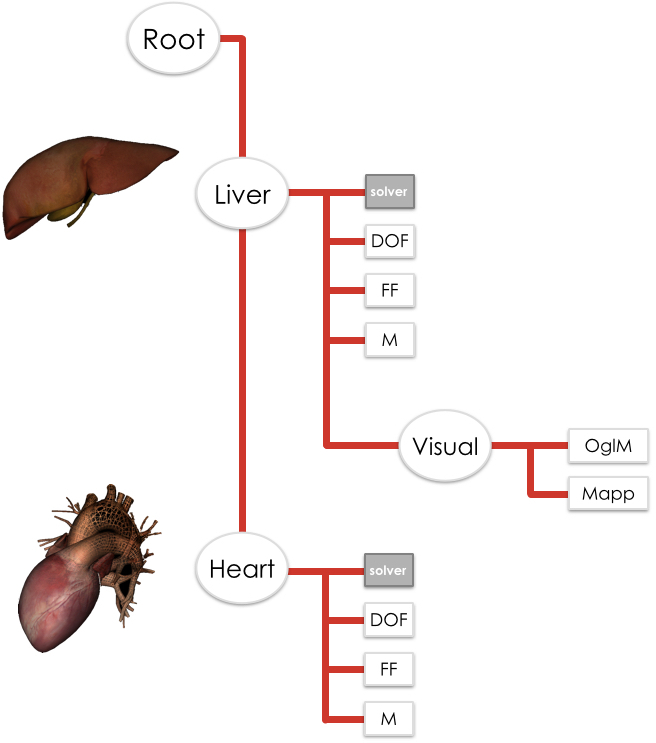
\includegraphics[width=\textwidth]{Sofa-graph}
    \caption[Example of SOFA scene graph]{SOFA representation of a scene with two objects: a liver and a
        heart. Each node of the scene can embed it's own set of solvers and
        visual representation.\\
        Image from SOFA documentation~\cite{SOFA16Sofa}.}
    \label{fig:sofa-tree}
\end{figure}

\subsection{Previous work on SOFA parallelisation}

It is important to note that the main developers of \gls{SOFA} are  mostly computer scientists with a physical or medical background but not specialized in \gls{HPC}.
Several efforts were made by external developers to parallelise \gls{SOFA}, most of these efforts consist in optimizing some algorithms which, according to \gls{SOFA} developers are costly in time.
For instance, Everton Hermann proposed an efficient (sequential) collision detection algorithm based on ray tracing and a parallelisation of this algorithm~\cite{Hermann08Raytraced}.
More recently, Julio Toss have been developing several algorithms on \glspl{GPU} to improve the computation time of Voronoi diagrams~\cite{Toss13Parallel,Toss14Parallel}.
These diagrams are critical for \gls{SOFA}, indeed while they allow to simulate efficiently the propagation of forces on heterogeneous materials~\cite{Faure11Sparse}, their computation generate a considerable overhead before the simulation.

Yet one limitation of this approach is that it can only optimize part of the code that are known to be slow.
Furthermore \gls{SOFA} is a generic framework, used among other things to develop new simulation algorithm, thus a suitable optimization should allow \gls{SOFA}'s developers to parallelize their code by themselves as they write it.

To overpass these limitations, E. Hermann exploited the hierarchy of the scene graph to parallelize the time integration step using the \gls{KAAPI} runtime~\cite{Gautier07KAAPI}.
This runtime allows to provide several implementations (\gls{CPU}, \gls{GPU} \ldots) for each task thus it can provide good performances on several machines with the same code.
Yet the amount of parallelisms depends of the number of objects on the scene graph thus scenes with only too few objects cannot benefit of this improvement.
Hence E. Hermann also designed a parallelisation based on domain decomposition for such scenes~\cite{Hermann09Interactive}.

While this approach is more generic and seems easier to generalize it was never actually used by \gls{SOFA} developers for several reasons: first of all they are not specialized on parallelism thus not used to work with runtimes such as \gls{KAAPI}.
Second \gls{KAAPI} is a research runtime that evolve quickly, therefore, the cost of maintaining code based on that runtime seems to important to them.
In the end, \gls{SOFA} is currently parallelized using simple \gls{OpenMP} \texttt{\#pragma} directives which allows to quickly parallelize a code, yet the result is considerably less efficient than the \gls{KAAPI} version.

To conclude it appears that optimizing algorithm pointed out by \gls{SOFA} developers is not enough as it can miss important part of the execution and it does not help them to writing parallel code.
Moreover a structural parallelisation relying on a research runtime may be discarded by them.
Hence, we should acquire a deep knowledge of \gls{SOFA} performances to identify hotspots and optimize the most important parts of the code and try to keep our optimization usable by the developers.

\section{Profiling tools}
\label{sec:prof-tools}

Performance analysis consists of to two steps: data collection and presentation.
The first step aims at extracting as much pertinent information from an execution as possible, yet observing an execution is not free: it takes time to count and record events thus it can impact the application performances or worst modify it's behavior.
Consequently, any analysis provides a trade-off between the amount of data collected and the impact on the monitored application.
The second step is also challenging as the tools needs to find out which data are pertinent and to present them in a meaningful way to the user.
Many tools were designed to address one or both of these challenges.

Performance counters, which were originally designed by \glspl{CPU} vendors to debug their processors prototypes, allows to count events such as cache miss, or branch miss-predict at a very low cost since they are hardware implemented.
They can directly be accessed using the \gls{Perf} driver which is part of the \gls{Linux} kernel since version $2.6.31$.
Yet as a result of their initial aim, the available counters depends of the \gls{CPU} model and vendor.
Furthermore it requires a deep knowledge of \glspl{CPU} mechanisms to understand the meaning of some counters.
Therefore higher level library such as \gls{PAPI}~\cite{Browne00Portable,Malony11Parallel,Weaver13PAPI} and \gls{Likwid}~\cite{Treibig10LIKWID} were designed to make it more convenient to access and interpret performance counters.
These libraries provides performance groups and automatically computes comprehensive metrics.
In addition they allow to start and stop the counters during the execution to focus on critical parts of the execution, which is useful once hotspot are identified, but can lead to miss a part of the execution if used too early.

An other approach to make performance counters more understandable consist on combining them with contextual informations obtained by hooking libraries calls (system calls, C standard library, \gls{MPI}, \gls{OpenMP} \ldots).
Such hooks can be deployed either by overwriting libraries calls at runtime with \texttt{LD\_PRELOAD} hack\footnote{One can use the \texttt{LD\_PRELOAD} environment variable to tell the linker to load a library before running a programming, allowing to intercept functions calls to external libraries such \texttt{malloc}}, or by using binary instrumentation libraries such as \gls{Intel} \gls{Pin}~\cite{Luk05Pin} or Dyninst from the Paradyn Project~\cite{Miller95Paradyn}.
The second method is more flexible and usually allows higher level data collection, yet it is more intrusive thus it can impact the behavior of the studied application.
Simulators such as \gls{SimGrid}~\cite{Casanova14Versatile} can be used to overpass these limitations, still they are usually more complex to install and use thus less likely to be adopted by developers from other fields than \gls{HPC}.
Several tools such as \gls{HPCToolkit}~\cite{Adhianto10HPCTOOLKIT}, \gls{PARAVER}~\cite{Pillet95PARAVER}, \gls{TAU}~\cite{Shende06Tau}, \gls{MAQAO}~\cite{Djoudi05MAQAO}, \gls{AMD} \gls{CodeXL}~\cite{AMD16CodeXL} (the successor of \gls{AMD} \gls{CodeAnalyst}~\cite{Drongowski08introduction}) and \gls{Intel} \gls{VTune}~\cite{Reinders05VTune} combines several of these methods to collects traces.

When it comes to presenting performance traces in a readable way, we can split these tools in three groups: the first one only provides textual traces and let the user extract pertinent informations from them.
This group includes the \gls{Perf} driver, \gls{Likwid} and \gls{PAPI} library as well as several \glspl{Pintool}.
Such traces are very useful for small applications as they do not require complex tools to be read, furthermore they are usually easy to parse thus one can build more complex visualisation upon it using \gls{R} for instance.
Tools from the second group, that includes\gls{VTune}, \gls{CodeXL} tries to present data in a more readable way, usually a set of tables and few plots, where they highlight values that seems to be pertinent (for instance cache miss above a fixed threshold) to help the user focusing on important parts.
Finally, while tools like \gls{MAQAO}, \gls{HPCToolkit} and \gls{PARAVER} propose visualisation similar too the second group by default, but they also provides \glspl{API} to design new visualizations or import external traces.
\gls{Framesoc}~\cite{Pagano13Trace} is very similar to the previous tools, the main difference is that it is designed for trace management and analysis, thus it does not provide any way to collect traces but it is able to import traces from several tools, it  describe them with a generic representation and allows to navigate easily through different visualizations of the same trace.

To conclude, many tools were developed to monitor an application's performance, the best tool depends of the kind issue we are looking for and the application we are monitoring.
Most of the tools discussed here are based on performance counters and therefore focus on the \gls{CPU}'s point of view.
In our specific case, we are studying a complex application, yet we are in contact with the developers of \gls{SOFA} thus the can give us hints on the important parts and the kind of issue we should look for.
Therefore low level tools such as \gls{Likwid} are well suited as they allow both to compute pertinent metrics and to focus on different part of the application.

\section{Experimental Methodology}
\label{sec:expe-methodo}

While in other domains such as biology experiments takes a large amount of time and money, they are almost inexpensive and can be designed very quickly in computer science.
As a results, we computer scientists, are not used to take the time to design correct experiments trying to minimize bias and using the right tools.
Furthermore as hardware and software evolves very quickly we usually does not bother to re run and verify the results presented previous studies while it is the best way to spot bias or confirm the validity of an experimental claim.

In this section we first introduce why reproducibility matters and how people have tried to reach it in \gls{HPC}, then we present the methodology we have developed during this thesis to make our experiment as reproducible as possible.


\subsection{Reproducible research}

Measurement bias, which means attributing a consequence to the wrong cause due to an issue in our measurement method, is a widely known phenomena in scientific communities and is analyzed in most fields.
Still in \gls{HPC} the only thing we usually do to avoid it is to run a large number of experiments hopping that if we have enough observations on several configurations the measurement bias will be negligible.
Mytkowicz et al.~\cite{Mytkowicz09Producing} highlighted several way to introduce significant measurement bias in computer science experiments without noticing it, showing that measurement bias is commonplace and unpredictable in our field.

As measurement bias is unpredictable even when we follow the best practices the easiest way to deal with it is to reproduce the study published by other team and confirm or invalidate their results.
While this is done in every scientific fields, it is not common to publish about experiment reproduction in \gls{HPC}.

A previous study~\cite{Collberg15Repeatability} tried to evaluate how reproducible the experiment presented in computer science article are.
To do so, they focused on the capacity to build the experimental code and evaluated $601$ articles published in “top ACM conferences and journal”.
From these $601$ articles they were only able to build the environment of $217$ articles.
Moreover it took more than half an hour to build $64$ of these papers and $23$ other required the intervention of the authors.

At this point we need to define precisely reproducibility, for the remaining
of this thesis, except if specified otherwise, we will use the definition
proposed by Dror G. Feitelson~\cite{Feitelson15From}:

\begin{quote}
    Repeatability concerns the exact repetition of an experiment, using the same experimental apparatus, and under the same conditions.

    Reproducibility is the reproduction of the gist of an experiment: implementing the same general idea, in a similar setting, with newly created appropriate experimental apparatus.
\end{quote}

It is nearly impossible to repeat an experiment in the exact same conditions as many exterior factors, such as the machine room temperature or the network usage done by other users on the same cluster, might impact the measured performances.
Still it is possible to repeat an experiment in similar conditions: someone who runs the same experiments two different days on the same machines can expect to obtain similar results.
Several tools can helps use making experiments more repeatable for instance by running our experiment on a shared platform such as grid5000~\cite{Cappello05Grid5000} we can hope that other people might access to the same set of machines.
Moreover deploying a custom environment on these machines allow to control and distribute the set of installed libraries.
Kameleon~\cite{Ruiz15Reconstructable} go even further as it allows to describe an environment as a recipe thus makes it easy to check the version of a library or replace it.

To reproduce an experiment it is important to understand how it has been designed and how it evolves from the first version to the results presented in the paper.
Stanisic et al.~\cite[Chapter~4, p31-44]{Stanisic15Reproducible} described an experimental workflow based on \gls{Git} and \gls{Org-mode} to keep track of these evolutions and make easy for someone to understand it.
One of the main drawback of this workflow is that it is not suitable for experiment which generate huge ($\ge$\SI{500}{Mib}) trace files as git is not designed to handle such files.

Several tools were designed to conduct experiments in computer science still they are not designed for \gls{HPC} and using them in our context would require some adjustments.
A more complete survey can be found in~\cite[Chapter~3, p17-19]{Stanisic15Reproducible}

\subsection{Experimental workflow}

We design experiments to answer simple questions such as ``Is my tool more efficient than the existing ones'', obviously this formulation is too vague to be answered scientifically.
We first need to find a set of relevant state of the art tools and then decide and on which configurations we are going to do the comparison.
This means choosing a set of benchmarks representing real life applications, one or several credible experimental machine(s).
Finally we must determine a set of metrics that we can measured accurately to evaluate the efficiency of the tools.

\begin{figure}[htb]
    \centering
    \includegraphics[width=\textwidth]{exp-tikz}
    \caption{Experimental pipeline}
    \label{fig:exp-pipeline}
\end{figure}

All these choices form a high level \emph{experimental plan}: it contains all the information required to reproduce the experiment but not to repeat it.
Indeed it miss the code that actually execute the experimental plan.
We can see an experiment as a pipeline that flow from this plan to the final human readable results as described in \fig{exp-pipeline}.
This pipeline is composed of three steps: the experimental plan that produce a (usually) huge set of data and meta data, the first one are meant to be used during the analysis while the second are only generated to find issues in the experiment or additional information to repeat it.
Then comes the raw analysis that extract pertinent information and compute metrics from the raw data.
The results of this step are usually easy to parse for a computer but not human friendly.
Thus the last step is there to present these data in a readable way.

Yet it is easy to present data in a tendentious way that reflects more our expectations than the reality without even noticing it.
To limit this bias, it is very important to design carefully the whole analysis before running the actual experiment and test the visualisation on a filler set of data.
Furthermore, adding comments to the visualisations about what they mean and what we expect to see can help reducing this bias.
Technologies such as \gls{R-markdown},Jupyter Notebook (anciently known as IPython Notebook) or \gls{Org-mode} are great help to produce reproducible experiments.

\subsubsection{Methodology}

\paragraph{Preparing an experiment:}

In this thesis, we ran two types of experiments: the fist one aims at analysing the behavior of one application (mostly \gls{SOFA}) while the second one aims at comparing trace collection tools.
For both analysis we need to find a set of \emph{benchmarks} to conduct our experiments, but the signification of this term is slightly different for the two cases.
In the first case, a benchmark is an input for the studied application and the set of benchmarks used should be defined with the developers of the application to cover the code that they want to improve.
While in the second case it means a set of applications which have a behavior representative of the applications targeted by the evaluated tool.
For this need, we use the \gls{npb}~\cite{Jin99NPBOpenMP} which allow to cover a large set of applications from simple computational kernels to real life applications.
Yet to compare several analysis tools, a set of benchmarks is not a sufficient input as these tools usually provides a large set of parameters allowing to modify their behavior, thus we must evaluate each tool under at least two set of parameters: the default and a tuned version with a set of parameters optimized for the results we are measuring.

Once the benchmarks are chosen, we need to decide of one machine or a set of machines on which we will run the experiment.
This step is crucial as computers architectures are getting more and more complex  and applications are (usually) designed for one type of machines.
Furthermore some tools (such as \gls{Pin}, \gls{PEBS}~\cite{Levinthal09Performance}, \gls{IBS}~\cite{Drongowski07Instructionbased}) are either vendor specific or optimized for some architecture.
Thus we must find machines that allow to do our study in a relevant situation and fair to the tools and libraries used.

Finally we need to find some relevant metrics to answer the questions that we are trying to answer with our experiment.
These metrics should remain simple as they will be interpreted by humans.
Yet they must also cover every aspects that we are studying.
A complete set of simple measurable metrics is often easier to understand that one complex metric that provide an overall score in an unknown unit.
Still simple ratios and percentages can make an analysis more reproducible for instance an execution time is significant only for a very specific configuration on one machine, while speedups and overheads can be compared more easily.


\paragraph{Writing the experiment scripts:}

It is crucial that any step of the experiment from the deployment of the
environment to the final analysis is properly scripted in a language that can
be understood by an other developer. Any manual step can make the experiment
impossible to repeat and an obscure code might make it hard to change some
parameters without breaking the whole experiment.

Furthermore the traces generated by an experiment must be self explanatory or
at some point they will only be a (large) set of meaningless bytes on a hard
drive. To do so it is important to keep with the data, the scripts
that generated it and the one that allows to interpret it. To do so, all our
experimental scripts starts the same way: they create a new directory that
will hold the traces, copy themselves and all the scripts which are on their
directory inside it. Then they duplicates their output to a file in this
experimental directory and Log every sensible meta data such as the
command that started the experiment, the machine name, its topology, \gls{OS}
the environment variables, the status of every dependencies (git version, diff
etc.). Such informations can be a great help to someone trying to reproduce
the experiment or to verify that the experimental condition are not biased.

An experiment consist of a set of independent runs, it is important to both
separate the execution of the runs and randomize their order. Indeed if
consecutive runs are part of the same program (i.e one loop that call several
time the same function instead of re-executing a program at each run), they
can benefit from cache effects. Moreover if the runs are randomized, external
(system) noise will either affect all runs are appears as chaotic, while if
they are ordered, it might be correlated with a parameter change.
Therefore our experimental scripts generate the list of runs that should be
executed shuffle it and then execute them in a randomized order. A run
consist of three step: a pre command that can set specific values,
the actual command that execute the benchmark and the post command that can
save and pre-process data, might compute metrics and must restore the normal state. Note that
the first and last steps are not mandatory. Each of the commands executed by
these 3 steps are logged before execution.

At the end of the day our experiment have produced a huge set of data that we
can divide on two categories: the meta data that are useful for debugging and
reproducibility and the raw results that will be filtered to then be analyzed.
The parsing step is designed only to extract data from the traces so the
analysis scripts can work on clean results, we avoid to do any statistic
during this step.

Finally for the analysis \gls{R} provides a large set of reliable statistic
analysis libraries and technologies such as \gls{R-markdown} or
\gls{Org-mode} allows to mix analysis code and results with comments. These
technologies allow to produce a standalone result (as a pdf or as a webpage)
that contains the original questions, our assumptions, the results and plots,
and our observation on these results.

\paragraph{Distributing the experiment:}

Trying to compile a badly documented code can be painful and time consuming,
the same problems occurs when it comes to reproduce experiment. Thus the
distribution of experiment traces and scripts must be considered carefully.
To repeat an experiment we need the scripts that run it, a description of the
machines and/or the virtual environment that is deployed and a link to the
right version of each tool, applications and benchmarks used during the
experiment. Several services such as Github, Bitbucked, and Gitlab \DBm{Urls
?} host freely code repositories, furthermore \glspl{VCS} such as \gls{Git}
\DBm{Citations ?} allow to track easily dependencies with a system of
submodules, therefore they are well suited for experiment distribution.
Finally an effort must be done on the documentation to help the user
understand why the experiment is designed, how it works and where (on which
machines) we should run it.

Distributing the experiment results can be more tricky as trace files can be
quite heavy and code repositories are usually not designed to handle large
files. While the experimental repository allows to repeat the whole
experiment, the trace distribution is useful to repeat only some specific
steps of the analysis, thus we distribute to set of files corresponding to the
two analysis steps depicted in \fig{exp-pipeline}. The first one contains all
the files generated by the experiment and the scripts to run that analysis.
This distribution can be quite heavy (around \SI{100}{Gib} for some of our
experiments) but allows to redo the whole analysis, compute new metrics or
look for additional informations in the meta data. At the opposite, the second
one only contains the filtered results and the scripts that generate the
plots, it allows to redo the statistical analysis exploring the data with a
different approach. Furthermore this trace usually contains more plots and
data than a published article that have to fit a certain amount of pages. Such
traces can be distributed using specialized large file hosting services such
as Renater File Sender, or Zenodo.\DBm{Url, Citation ?}


\section{SOFA Analysis}
\label{sec:sofa}

In this section, we present first the experiment designed to produce a performance analysis of \gls{SOFA}, then we discuss the obtained result on the possibility of improvements.

\subsection{Experiments}

The current version of \gls{SOFA} is mostly sequential code with a simple \gls{OpenMP} parallelization.
Yet this parallelization is known to be often not efficient.
The \gls{SOFA} developers gave us $4$ simulation scenes specifically designed to test the most popular part of \gls{SOFA}.
Moreover they give us hints of function that are known as hotspots.

We decided to use \gls{Likwid} to analyze \gls{SOFA} performances as it is quite flexible allowing both global (wrapper mode) and local (marker mode) analysis and provides several useful metrics and performance groups out of the box.

More specifically, we focused the following metrics:
\begin{itemize}
    \item \emph{Idle time ratio}: The CPU is idle when it is waiting for a transfer to memory,  disc or network \gls{I/O}.
        Idle time can often be reduced either by overlapping it with computation or by improving memory (or \gls{I/O} access pattern).
        This metric gives the ratio between the time spent idel and the time actually spent computing things during the simulation.
    \item \emph{Simulation time}: The time spend inside \gls{SOFA} simulation loop, this is only useful to compare parallel execution to sequential ones.
    \item \emph{Runtime ratio}: For each function, the ratio of the time spend in this function and the total time spent in the simulation loop.
        This metrics show if a function is a hotspot or not.
    \item \texttt{L2}, \texttt{L3} and \texttt{MEM} predefined groups from \gls{Likwid}. These groups compute mainly the data volume exchanged at their level level (respectively second level of cache, third level of cache and main memory) and the bandwidth.
        These two metrics and more precisely their evolution between sequential and parallel executions tells us how much data is shared between the threads and if it shared efficiently or not.
        These metrics are computed by counting the misses at the lower level (hence the absence of \texttt{L1} group).
\end{itemize}

\begin{table}[t]
    \centering
    \begin{tabular}{lccccc}
        \toprule
        \multirow{2}{2cm}{CPU} & Vendor & Model & Core & Threads & Frequency \\
        \cmidrule(lr){2-6}
        & Intel & Xeon E5-1607 & $4$ & $4$ & \SI{3.00}{Ghz} \\
        \midrule
        \multirow{3}{2cm}{Cache\\and\\Memory} & L1 & L2 & & L3 & Memory \\
        \cmidrule(lr){2-6}
        & \multicolumn{2}{c}{Private} & & \multicolumn{2}{c}{Shared} \\
        \cmidrule(lr){2-3}
        \cmidrule(lr){5-6}
        & \SI{32}{Kib} & \SI{256}{Kib} & &\SI{10}{Mib} & \SI{16}{Gib} \\
        \bottomrule
    \end{tabular}
    \caption{Hardware configuration of Hopi.}
    \label{tab:hopi-hw}
\end{table}

As \gls{SOFA} is mainly used on personal machines and not \gls{HPC} ones, we ran our performance evaluation on a recent desktop machine called \emph{Hopi} (formerly known as \emph{Naskapi}).
The hardware specifications of this machine are described in \tbl{hopi-hw}.
It runs a \gls{Debian} \emph{Wheezy} on a Linux kernel $3.2.0$-$4$ with hyper threading disabled.

The experimental methodology described in \sect{expe-methodo} evolved during this Ph.D thesis, hence the experiments presented here does not fit it perfectly, the main mistake is that we did not made an image of our experimental system, furthermore the runs were independent but not randomized.


\subsection{Results and Discussions}

To present the results of our evaluation, we will focus on two \gls{SOFA} scenes that illustrate the kind of results we obtained.
The first scene is called \emph{linearQuadraticFrame}, for this scene the \gls{OpenMP} parallelisation provides a speedup of $1.37$ with four threads which is clearly not optimal.
Yet compared to the second scene \emph{linearRigidAndAffineFrame}, which has a speedup of $0.87$, it seems efficient.
Thus our first goal was to understand why while some scenes takes advantage of this parallelisation some other are slowed down by it.

Before digging into the differences between these scenes, there are two noticeable similarities between them to discuss.
First the idle time ratio reported by \gls{Likwid} showed that, for the sequential version of the code, during almost half of the simulation the processor is idle, which means that we spend a lot of time waiting for \gls{I/O} or memory accesses.
In parallel  this idle time increases, yet this behavior is expected as the \gls{OpenMP} based parallelisation only affect some small parts of the code, hence as soon as we are not in a parallel loop, $3$ threads out of $4$ are idle.
The second noticeable similarity is that the functions pointed by the developers only represent around \SI{30}{\%} of the simulation time, which means that there are some unknown hotspots left.

From here, we know that there might be a memory issue (as the processor spend a lot of time idle), and we have two scenes: one where the parallelisation speed the execution up and one on which it slows it down.
We compared the bandwidth and data volume from the \texttt{L2} cache to the main memory for the two scenes and for the functions indicated by the developers.
Those functions are generic and thus their actual code varies depending on the parameters of the simulation.
Therefore while the compared functions are similar in terms of role in the simulation, the manipulated data as well as the executed code is different for the two scenes.

\begin{figure}[htb]
    \centering
    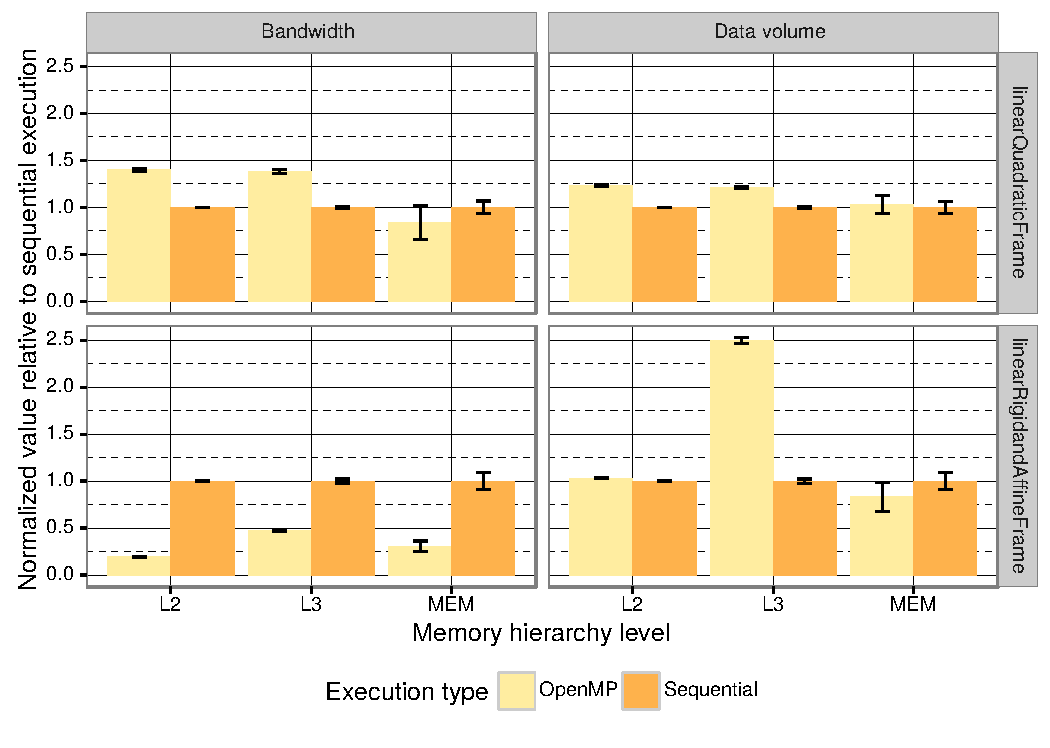
\includegraphics[width=\textwidth]{SOFA_perfctr.pdf}
    \caption[SOFA likwid results]{Differences of bandwidth and data volume, from L2 cache to main memory, between sequential and parallel execution of \gls{SOFA} on two different simulation scenes.
        \\
        For both bandwidth and data volume, the value is normalized to the mean value of the corresponding sequential executions.
        \\
        For bandwidth, higher is better while for data volume lower is better.
    }
    \label{fig:SOFA-perfctr}
\end{figure}

\fig{SOFA-perfctr} shows the bandwidth (left side) and the data volume (right sides) for the two functions (\emph{linearQuadraticFrame} above, \emph{linearRigidAndAffineFrame} below) from \texttt{L2} cache to the main memory.
Each point represents the mean of $60$ runs and the error bars represents the standard error.
To make the plot more readable, we've normalized each value by dividing it by the value for the corresponding sequential run, thus these plots show the evolution of the bandwidth and data volume when we use the \gls{OpenMP} version of\gls{SOFA}.

We can see that for the first scene, both the bandwidth and data volume increases by a factor of $1.5$ in the cache and stays comparable in the main memory when we use the parallel version.
This means that the thread are either sharing efficiently data or at least working on data different enough to not step on each other foots.
At the opposite for the second scene, the bandwidth drops down at each level and the data volume stays still except at the \texttt{L3} level where it increases by a factor $2.5$.
It is important to note that the \texttt{L3} cache is the only shared cache which means that a considerable amount of data is invalidated in \texttt{L2}, in other words, several threads are writing the same data, invalidating each other private cache and requiring the coherency protocol to interfere.
This behavior is called false sharing and is a well known performance issue.

At this point we can say that false sharing occurs on this precise function, yet we don't know on which data structure.
We could dig onto the code and try to understand the memory access pattern of each data structure to see where the false sharing does occurs.
By looking at \gls{SOFA}'s code, we can see that the main difference between the two version of the function is that for \texttt{linearRigidAndAffineFrame} there is one more loop in the computation.
Still this code manipulate several data through many indirections, therefore determining on which data the false sharing is happening could be extremely slow.
Furthermore this approach is not generic at all, and once we've done it for one particular function, we would have to redo the same analysis and optimization for each potential hotspot.

Furthermore as we have seen with the runtime ratio, this particular false sharing issue only represent a small part of the execution, therefore a more generic approach would be welcome.

From that point it seems clear that \gls{SOFA} is having memory performance issues, yet we need a generic tools to analyze its performances from the memory point of view.
Such tool should be able to show the memory access patterns of each thread over the different data structures and point us through patterns that are (or can be) inefficient.

% vim:set et si sta lbr  sw=4 ts=4 
